\documentclass{article}\usepackage[]{graphicx}\usepackage[]{color}
%% maxwidth is the original width if it is less than linewidth
%% otherwise use linewidth (to make sure the graphics do not exceed the margin)
\makeatletter
\def\maxwidth{ %
  \ifdim\Gin@nat@width>\linewidth
    \linewidth
  \else
    \Gin@nat@width
  \fi
}
\makeatother

\definecolor{fgcolor}{rgb}{0.345, 0.345, 0.345}
\newcommand{\hlnum}[1]{\textcolor[rgb]{0.686,0.059,0.569}{#1}}%
\newcommand{\hlstr}[1]{\textcolor[rgb]{0.192,0.494,0.8}{#1}}%
\newcommand{\hlcom}[1]{\textcolor[rgb]{0.678,0.584,0.686}{\textit{#1}}}%
\newcommand{\hlopt}[1]{\textcolor[rgb]{0,0,0}{#1}}%
\newcommand{\hlstd}[1]{\textcolor[rgb]{0.345,0.345,0.345}{#1}}%
\newcommand{\hlkwa}[1]{\textcolor[rgb]{0.161,0.373,0.58}{\textbf{#1}}}%
\newcommand{\hlkwb}[1]{\textcolor[rgb]{0.69,0.353,0.396}{#1}}%
\newcommand{\hlkwc}[1]{\textcolor[rgb]{0.333,0.667,0.333}{#1}}%
\newcommand{\hlkwd}[1]{\textcolor[rgb]{0.737,0.353,0.396}{\textbf{#1}}}%

\usepackage{framed}
\makeatletter
\newenvironment{kframe}{%
 \def\at@end@of@kframe{}%
 \ifinner\ifhmode%
  \def\at@end@of@kframe{\end{minipage}}%
  \begin{minipage}{\columnwidth}%
 \fi\fi%
 \def\FrameCommand##1{\hskip\@totalleftmargin \hskip-\fboxsep
 \colorbox{shadecolor}{##1}\hskip-\fboxsep
     % There is no \\@totalrightmargin, so:
     \hskip-\linewidth \hskip-\@totalleftmargin \hskip\columnwidth}%
 \MakeFramed {\advance\hsize-\width
   \@totalleftmargin\z@ \linewidth\hsize
   \@setminipage}}%
 {\par\unskip\endMakeFramed%
 \at@end@of@kframe}
\makeatother

\definecolor{shadecolor}{rgb}{.97, .97, .97}
\definecolor{messagecolor}{rgb}{0, 0, 0}
\definecolor{warningcolor}{rgb}{1, 0, 1}
\definecolor{errorcolor}{rgb}{1, 0, 0}
\newenvironment{knitrout}{}{} % an empty environment to be redefined in TeX

\usepackage{alltt}
\usepackage[margin=1in]{geometry}
\usepackage{amsmath}
\usepackage{amssymb}
\usepackage{graphicx}
\usepackage{float}
\usepackage{hyperref}

%% <<setup, include=FALSE>>=
%% library(highr)
%% knit_hooks$set(inline = function(x) {
%%   if (is.numeric(x)) return(knitr:::format_sci(x, 'latex'))
%%   highr:::hi_latex(x)
%% })
%% @
%% % The above is supposed to enable inline code highlighting using \Sexpr{},
%% % but i can't get it to work; just , does the same thing as \texttt{}. My tester is on line 58
\IfFileExists{upquote.sty}{\usepackage{upquote}}{}
\begin{document}
%% \SweaveOpts{concordance=TRUE}
\title{Bayesian Analysis in AD Model Builder}
\author{Cole C. Monnahan | monnahc@uw.edu \\
Peter T. Kuriyama | ptrkrym@uw.edu}

\date{\today{}}
\maketitle
\begin{abstract}
  The goal of this guide is to outline and describe the steps needed to conduct a Bayesian analysis in AD 
  Model Builder. Included are general descriptions of Bayesian inference, Priors, and two MCMC algorithms. We
  hope that the guide will enable users to take fuller advantage of the features of ADMB that are built in
  but not well-documented.
  
\end{abstract}

\tableofcontents

\section{Introduction}
  The goal of this guide is to outline and describe the steps needed to conduct a Bayesian analysis in AD 
  Model Builder. Included are general descriptions of Bayesian inference, Priors, and two MCMC algorithms. We
  hope that the guide will enable users to take fuller advantage of the features of ADMB that are built in
  but not well-documented.

  AD Model Builder is the fastest, most powerful software for fitting general nonlinear statistical models.
  The "AD" refers to automatic differentiation that comes from a C++ library which implements reverse mode 
  automatic differentiation. 
  
-Add short paragraph about r2admb package

  We encourage others to contribute to this guide and further document the Bayesian capabilites of ADMB.
  The contents of this document available on a \href{https://github.com/colemonnahan/admb_guide}{github
  repository} maintained by Cole Monnahan. 
  
  Something about about where to make code suggestions?
  
  
\section{Bayesian inference}
In general, Bayesian inference is used to quantify the full
range of uncertainty around both models and parameter values
and incorporate findings from historical studies. In a
fisheries specific context, Bayesian inference allows
scientists to investigate the consequences of alternative
management strategies.

Markov chain Monte Carlo (MCMC) is a common algorithm used
to sample and compute expectations with respect to complex
and high-dimensional probability distributions.  ADMB
implements two different MCMC algorithms: the ubiqitous
Metropolis-Hastings and a Hamiltonian (or ``hybrid'')
sampler, both described in this section.

John Kruschke in ``Doing Bayesian Data Analysis: A Tutorial
with R and BUGS'' has a simple example that illustrates the
mechanics of the Metropolis-Hastings algorithm. A politician
lives on a long chain of islands. The politician's goal is
to stay in the public eye by traveling to each island
proportional to their relative population. In other words,
he will spend more time on highly populated islands and less
time on less populated islands. He flips a fair coin to
propose a move to an island east or west of his current
location. If the proposed island has a higher population
than his current island he moves. If the proposed island has
a smaller population than his current island he will only
move with a probability $P_{proposed} / P_{current}$ where
$P_{proposed}$ is the population of the proposed island and
$P_{current}$ is the population of the current island.

All MCMC algorithms work in this same general way. The user
will start the algorithm at an arbitrary starting point, and
the algorithm will propose new parameter sets or states. The
algorithm will propose new states (i.e. parameter draws) and
move to that state, or not, depending on its density
relative to the current state. Just like the politician, the
algorithm will spend most of the time in states with high
densities.

MCMC algorithms typically need a ``burn-in'' period,
especially if the starting point is in a region with low
density. The goal of a MCMC algorithm is to explore areas
with the highest probabilities in a distribution. It will
perhaps take thousands of draws for the algorithm to find
the peaks of the distribution, especially if it starts in a
low density region. Discarding these intial draws allows the
algorithm to explore the main regions of the target
distribution.

Autocorrelated MCMC samples are close together and probably
not a true represenation of the underlying
distribution. Samples are typically ``thinned'' every
nth-step to generate uncorrelated samples. The tradeoff is
that excessive thinning increases run-time for the
algorithm.

The R package \texttt{CODA} is a commonly used tool for
checking MCMC diagnostics such as autocorrelation.

\section{Priors}
As with any Bayesian analysis, priors are a key component of
the posterior surface and must be considered in ADMB as
well. The posterior density is proportional to the product
of the likelihood and priors. ADMB works in the negative log
space, so he contribution of priors is incorporated into the
model by adding the negative log of the prior density to the
objective function. At this point the minimum point is no
longer the maximum likelihood estimate, but rather what we
refer to as the ``maximum posterior mode''-- i.e. the
parameters corresponding to the highest point of the
posterior. The difference between the two is subtle, but
there are important philosophical differences: with Bayesian
analysis ADMB is integrating across the parameter space,
while the likelihood framework focuses on maximization.

The way MCMC works in ADMB, users need not explicitly define
and incorporate priors into their model. In this case
``implicit'' priors are still affecting the posterior. In
particular, unbounded parameters without explicit priors
have infinitely broad uniform priors (an example of an
``improper'' prior because it will not integrate to
1). Another example is a variance parameter estimated in log
space and then exponentiated within the model to keep it
above zero. An implicit uniform prior on the log parameter
may not be uninformative on the natural scale. The
implications of these issues are contentious and certainly
beyond the scope of this guide. We caution users to
carefully consider and explicitly acknowledge their priors
-- ADMB will not force you to.

Uniform priors can be incorporated without changing the
objective function calculation by bounding the
parameter. Other forms of prior distributions need to be
added manually by the user, with our without any
constants. For instance, a normal ($N(5,1)$) prior on a
parameter $a$ could be added as
\texttt{f+=pow((a-5),2)/(2*1*1)}, where the constants have
been dropped.

\section{Markov chain Monte Carlo (MCMC) in ADMB}
Markov chain Monte Carlo (MCMC) is a common algorithm used
to sample from arbitrary, unscaled posterior
distributions. ADMB implements two different MCMC
algorithms: the ubiqitous Metropolis-Hastings and a
Hamiltonian (or ``hybrid'') sampler, both described briefly
below.

All MCMC algorithms work by proposing new states
(i.e. parameter vectors) and moving to that state, or not,
depending on its density relative to the current state. The
algorithm thus generates series of autocorrelated parameter
vectors which can be thinned to produce independent samples
from the posterior distribution of interest.

\subsection{Workflow}
The R package \texttt{R2admb} contains some useful functions
for streamlining the workflow of MCMC in ADMB. For users who
wish to have more manual control, the following steps
outline a typical workflow.
\begin{enumerate}
\item Build, run, and verify an ADMB model. This model must
  explicitly include the contribution of the priors to the
  objective function, such that the ADMB estimate is the
  posterior mode, rather than a maximum likelihood estimate.
\item Run an MCMC using the command line argument
  \texttt{-mcmc $N$ -mcsave $N_{\text{save}}$} (among other
  options, see below). The thinned draws are discarded,
  leaving a total of $N_{\text{out}}=N/N_{\text{save}}$
  saved draws. For example \texttt{-mcmc 1e6 -mcsave 1000}
  will run 1 million draws but only save (i.e.``thin'')
  every 1000th, for a total kept of $Nout=1000$.
\item After completion, run the model again with argument
  \texttt{-mceval}. This command tells ADMB to loop through
  the saved iterations (in the \texttt{.psv} file) and
  execute in the \texttt{mceval\_phase()}.
\item Pull results into R or other program to ensure the
  sample is sufficiently thinned, either visually or with
  tools using, for example, the \texttt{CODA} package.
\item If necessary, rerun the chain with more thinning, drop
  the first part of the chain as a ``burn-in,'' or run
  longer for more iterations.
\item Make whatever Bayesian inference is desired using the
  $Nout$ independent samples.
\end{enumerate}

\subsection{MCMC Phases}
ADMB is designed with two phases that are used to produce
MCMC output: (1) the \texttt{mcmc} phase and (2)
\texttt{mceval} phase. While the use of these phases is not
common (is this true??) among other MCMC software, and may
be a source of confusion for new ADMB users, they provide a
powerful and efficient framework for MCMC analyses.

The \texttt{mcmc} phase is the one with which most people
are already familiar. This is where ADMB generates new
parameter sets by proposing a set, and then determining
whether to move there or stay at the current set. This
process is repeated $N$ times, and how sets are proposed
depend on the algorithm used (see section \ref{sec:MH} and
\ref{sec:hybrid}). During this phase, the $Nout$ saved
parameter values are written to a \texttt{.psv} file
(described below). Note that if \texttt{-mcsave $nsave$} is
not specified, ADMB will run the MCMC but no values will be
saved.

The \texttt{mceval} is an optional phase that is designed to
be run after the \texttt{.psv} file has been
produced. During this phase, ADMB loops through the $Nout$
parameter combinations in the \texttt{.psv} file and reruns
the \texttt{PROCEDURE\_SECTION} in the \texttt{mceval()}
phase. This phase is extremely powerful because it allows
the user to minimize wasted calculations by parsing
calculations into two groups: those that affect the
objective function (i.e. posterior calculations for Bayesian
analyses) and those that do not. Calculations done for
discarded draws (which often is most iterations) simply slow
down the analysis. Thus, an analysis can be made to run
faster by minimizing calculations in the \texttt{mcmc}
phase.  For example, a user may want to extrapolate
(e.g. project a time series into the future) or calculate
values derived from the parameters and intermediate
values. By putting these calculations inside an
\texttt{mceval\_phase} clause they are only done for saved
draws and the MCMC will run faster. In practice, some chains
need to be thinned significantly more than 1 in 1000, so the
time saved can be substantial, especially if the
\texttt{mceval\_phase} calculations are time-consuming.

While the \texttt{mceval} phase was designed specifically
for MCMC analyses, it can be coopted for use in other types
of analyses. In essence it is a convenient framework in
which to get ADMB to quickly evaluate arbitrary sets of
parameters, while only initializing once. Examples of
alternative uses are the SIR algorithm,
evaluating a grid of points for plotting and exploration of
the posterior surface, or trying random parameter sets to
investigate local minima. Getting ADMB to evaluate these
parameter sets is as simple as writing them to the
\texttt{.psv} file and then executing ADMB with the option
\texttt{-mceval}. See section (\ref{sec:outfiles}) for
details on how to do this.


\subsection{Output files}\label{sec:outfiles}
\subsubsection{Meta data: The hst file}
Melissa todo
\subsubsection{Parameter draws: The psv file}
During the \texttt{mcmc} phase, saved parameter values, in
bounded space, are written to a binary file called
\texttt{<model name>.psv}. This file can be read into R
using the following commands:
\begin{knitrout}
\definecolor{shadecolor}{rgb}{0.969, 0.969, 0.969}\color{fgcolor}\begin{kframe}
\begin{alltt}
psv <- \hlkwd{file}(\hlstr{"<model name>.psv"}, \hlstr{"rb"})
nparams <- \hlkwd{readBin}(psv, \hlstr{"integer"}, n=1)
mcmc <- \hlkwd{matrix}(\hlkwd{readBin}(psv, \hlstr{"numeric"}, n=nparams*<Nout>), ncol=nparams, byrow=TRUE)
\hlkwd{close}(psv)
\end{alltt}
\end{kframe}
\end{knitrout}
The first element in the \texttt{.psv} file is the number of
active parameters in the model, which then tells R how to
parse the following elements into parameter values. Note
that the value of $Nout$ in \texttt{nparams*Nout} depends on
\texttt{Nmcmc} and \texttt{mcsave} and must be specified
manually. This is the main file that was designed to be used
to extract MCMC draws from ADMB. However, this file only
contains parameter values and not derived quantities or
other quantities of interest (e.g. $MSY$ or biomass
trajectories) which often are of interest.
\subsubsection{Derived quantity draws}
Often the posterior distribution for quantities other than
the parameters are desired. Examples of derived quantities
are: functions of parameters, properties of the model, or
model projections/extrapolations.

A simple way of extracting this information is to bypass the
\texttt{psv} file altogether and use a \texttt{C++} function
to write a \texttt{.csv} file containing whatever elements
are desired. This can be accomplished inside the ADMB
\texttt{.tpl} file with just a few lines of code. Inside the
\texttt{DATA\_SECTION} section use the following code to
create an IO object that writes values to a \texttt{.csv}
file, similar to the function \texttt{cout} which prints to
screen.
\begin{knitrout}
\definecolor{shadecolor}{rgb}{0.969, 0.969, 0.969}\color{fgcolor}\begin{kframe}
\begin{alltt}
  !!CLASS ofstream \hlkwd{MCMCreport}(\hlstr{"MCMCreport.csv"},ios::trunc);
\end{alltt}
\end{kframe}
\end{knitrout}
Then, inside the \texttt{PROCEDURE\_SECTION} the function
can be used to write both parameters, derived quantities, or
other information about the model.
\begin{knitrout}
\definecolor{shadecolor}{rgb}{0.969, 0.969, 0.969}\color{fgcolor}\begin{kframe}
\begin{alltt}
  \hlkwd{if}(\hlkwd{mceval_phase}())\{
    \hlkwd{if}(header==1) \{
        MCMCreport << \hlstr{"a,b,NLL,ab"} << endl;
        header=0;
    \}
    MCMCreport << a <<\hlstr{","} << b << \hlstr{","} << NLL << \hlstr{","} << ab << endl;
  \}
\end{alltt}
\end{kframe}
\end{knitrout}

In this case the parameters $a$ and $b$ are saved, along with the negative
log-likelihood and product of the model parameters.  The
\texttt{MCMCreport} object is used just like \texttt{cout} and is executed
only during the \texttt{mceval} phase so that only saved values are written
to the file as ADMB iterates through each saved parameter. The variable
header is set to 1 in the \texttt{GLOBALS\_SECTION} as \texttt{int header =
  1;}. Naturally this code can be used anywhere in the procedure section,
and this may be a useful diagnostic tool in some situations. The file is
recreated at each execution if \texttt{ios::trunc} is used, or it can be
appended with \texttt{ios::app}. New draws are appended to the
\texttt{MCMCreport.csv} file so that it must be deleted in between MCMC
runs.

\subsection{Convergence diagnostics} \label{sec:diag}
Burn-in and thinning, how to check this? What happens if not
independent?

\subsection{Resuming a chain}\label{sec:restart}
The MC resume command, \texttt{-mcr}, allows the user continue sampling along 
a previuosly run MCMC chain. Say that the user has run a chain, checked diagnostics, and 
concluded that the chain needs to thinned further as samples appear to be correlated.
Rather than restarting a new chain, the user can save computation time by using \texttt{-mcr} 
to pick up an existing chain where it left off. 

Resuming a chain is simple, and only requires \texttt{-mcr} to an MCMC statement. 
Let's save ten values from a chain, saving every 20th value with a seed of 30.

\begin{verbatim}
simple -mcmc 200 -mcsave 20 -mcseed 30
\end{verbatim}

Now say that we want to thin the chain, saving every 50 values until we have
additional values. Modifying the number of iterations, values to save and adding \texttt{-mcr} and 
\texttt{-nosdmcmc} (per the ADMB manual) will achieve this. 

\begin{verbatim}
simple -mcmc 500 -mcsave 50 -mcr -nosdmcmc
\end{verbatim}

The saved parameter values from the first and resumed chain are shown in Table 1. The first ten values from
the first chain and the resumed chain are identical as expected. 

Adding the command \texttt{-noest} can save further computation time as minimization is not necessary. 


\begin{table}[ht]
\centering
\begin{tabular}{r r r r r}
  \hline & a-first & b-first & a-resumed & b-resumed \\ 
  \hline
  1 & 1.91 & 4.08 & 1.91 & 4.08 \\ 
  2 & 2.00 & 4.78 & 2.00 & 4.78 \\ 
  3 & 2.08 & 3.40 & 2.08 & 3.40 \\ 
  4 & 1.85 & 4.35 & 1.85 & 4.35 \\ 
  5 & 1.88 & 4.31 & 1.88 & 4.31 \\ 
  6 & 1.86 & 4.94 & 1.86 & 4.94 \\ 
  7 & 1.89 & 2.18 & 1.89 & 2.18 \\ 
  8 & 2.62 & 0.78 & 2.62 & 0.78 \\ 
  9 & 2.16 & 2.99 & 2.16 & 2.99 \\ 
  10 & 1.94 & 3.49 & 1.94 & 3.49 \\ 
  11 & 0.00 & 0.00 & 0.33 & -1.25 \\ 
  12 & 0.00 & 0.00 & 1.75 & 4.59 \\ 
  13 & 0.00 & 0.00 & 1.74 & 4.80 \\ 
  14 & 0.00 & 0.00 & 1.94 & 2.62 \\ 
  15 & 0.00 & 0.00 & 2.16 & 3.08 \\ 
  16 & 0.00 & 0.00 & 1.99 & 4.18 \\ 
  17 & 0.00 & 0.00 & 2.09 & 2.95 \\ 
  18 & 0.00 & 0.00 & 1.94 & 4.17 \\ 
  19 & 0.00 & 0.00 & 1.52 & 5.87 \\ 
  20 & 0.00 & 0.00 & 1.91 & 4.38 \\ 
   \hline
\end{tabular}
\caption{Parameter values from an example MCMC chain and the resumed MCMC chain}
\label{tab:mcr_table}
\end{table}



%%# <<makeTable, eval=TRUE, echo=FALSE, results = 'asis', warning = FALSE, message = FALSE >>=
%%# setwd('/Users/peterkuriyama/School/Research/admb_guide/examples/simple')
%%# source('mcr_test_main.r')
%%# 
%%# out <- check_mcr(Nout = 10, mcsave = 20, mcseed = 30,
%%#           Nout.mcr = 10, mcsave.mcr = 40) 
%%# 
%%# print(xtable(out))
%%# @

\subsection{Starting values}\label{sec:startvals}
For many Bayesian software platforms, the MCMC algorithms
are started at user-chosen or arbitrary places. ADMB has the
advantage that it can robustly estimate the posterior mode
and the covariance at that point. This information is very
valuable in initializing the MCMC chain.

Specifically, an MCMC chain starts from the posterior mode
and uses the estimated covariance matrix in its proposed
jumps (see the algorithm sections below). As such, ADMB
chains typically do not need a long period to reach areas of
high density.

The user can specify starting values via the command line
option \texttt{mcpin <file>} which must point to a file with
starting values for parameters.



\section{Metropolis-Hastings MCMC}\label{sec:MH}
The default MCMC algorithm used by ADMB is the
Metropolis-Hastings (MH) algorithm\footnote{Technically it
  has a symmetric proposal, a special case known as the
  Metropolis algorithm.}. This algorithm has been around for
decades, is simple to implement and used widely.

This algorithm will be most efficient when the posterior
surface mimics a multivariate Normal distribution.

\subsection{Algorithm}
Let
\begin{align*}
  f&=\text{the ADMB objective function}\\
  c&=\text{an unknown normalization constant}\\
  Xcur&=\text{current parameter vector}\\
  Xprop&=\text{a proposed parameter vector}\\
  U&=\text{a randomly drawn uniform value in [0,1]}\\
\end{align*}
Then
\begin{equation}
  Xnew=
  \begin{cases}
    Xprop & \text{if} \quad U\leq \dfrac{cf(Xprop)}{cf(Xcur)}\\
    Xcur & \text{otherwise}
  \end{cases}
\end{equation}
The proposal (or ``jump'') function proposes new parameter
vectors given the current set. The default behavior for ADMB
is to use a multivariate normal
distribution\footnote{Technically a bounded multivariate
  normal, operating in a transformed parameter space via the
  Cholesky decomposition of the covariance matrix, but we
  ignore that here for simplicity and clarity.} centered at
the current vector:
\begin{equation*}
  Xprop\sim MVN(Xcur, \Sigma)
\end{equation*}
 where $\Sigma$ is the covariance matrix obtained by
 inverting the Hessian at the posterior mode.

\subsection{MCMC Arguments}
ADMB has a suite of arguments available to the user at run
time. We cover the most commonly used ones, and refer the
user to the ADMB manual and other documentation for further
options.
\begin{table}[h]
  \centering
  \begin{tabular}[h]{|cl|}
    \hline
    \texttt{-mcmc N} & Run $N$ MCMC iterations\\
    \texttt{-mcsave N} & Save every $N$th MCMC iteration\\
    \texttt{-mcscale N} & Rescale step size for first $N$ iterations\\
    \texttt{-mcmult N} & Rescale the covariance matrix\\
    \texttt{-mcpin <file>} & Start algorithm from values in <file>\\
    \texttt{-mcrb N} & Reduce high parameter correlations
    (see \ref{sec:mcrb})\\
    \texttt{-mcprobe X} & Use a fat-tailed proposal
    distribution (see \ref{sec:mcprobe})\\
    \texttt{-mcdiag} & Use a diagonal covariance matrix\\
    \texttt{-mcnoscale} & Do not scale the algorithm during\\
    \texttt{-mcscale N} & Scale the algorithm during the
        first $N$ iterations\\
    \texttt{-mcu} & Use a uniform distribution as proposal distribution.\\
    \hline
  \end{tabular}
  \caption{ADMB runtime arguments for the Metropolis-Hastings MCMC}
  \label{tab:mh_args}
\end{table}
\subsection{Console output}
When running an MCMC chain from the console, the output
similar to the following will appear.
\begin{verbatim}
Initial seed value -36519
-14.9642 -14.9642
 mcmc sim 1  acceptance rate 0 0
-15.4843 -15.4843
 mcmc sim 201  acceptance rate 0.517413 0.52
increasing step size -1.32761
-15.7798 -15.7798
 mcmc sim 401  acceptance rate 0.428928 0.34
\end{verbatim}
ADMB prints the random seed used, and then the negative
objective function value twice. In this case scaling is
increased after the first 200 iterations (proposing more
distant values). This is followed by the log of the
determinant of the Choleski decomposed covariance matrix. In
some cases this information may be useful for
troubleshooting, but for most practical purposes it can be
ignored.
\subsection{Example MCMC}
We demonstrate these concepts using the ``simple'' model
packaged with ADMB, which is a contrived two parameter
linear model ($y=ax+b$). First we run the model without any
thinning by specifying \texttt{mcsave}=1 (figure
\ref{fig:simple1}).
\begin{figure}[h]
  \centering
  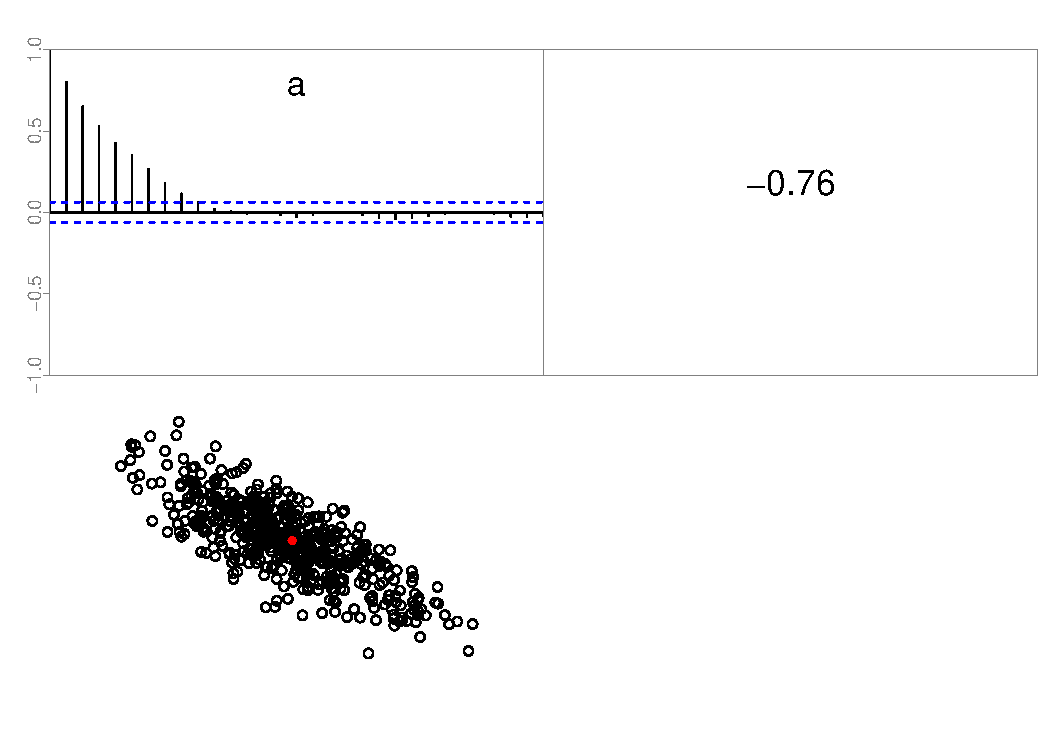
\includegraphics[width=5in]{../plots/simple1.pdf}
  \caption{The samples from a simple model with
    \texttt{mcsave}=1. Note the high autocorrelation of both
    parameters.The red ellipses show the estimated pairwise
    parameter covariances, and the red point the MPD.}
  \label{fig:simple1}
\end{figure}
The MCMC chain is clearly autocorrelated from the acf plots
and the traces (not show). This chain needs to be tuned to
achieve independent samples.
\subsection{Tuning the MH algorithm}
The goal of ``tuning'' the algorithm is to obtain
independent samples from the posterior, with as few of
calculations as possible (to keep runtime manageable). For
the MH algorithm, there are several ways the user can tune a chain.

\subsubsection{Thinning rate}
For the MH algorithm, the most important tuning option
available to the user is the thinning rate. This is the rate
at which parameters are saved, such that thinning is
effectively discarding draws. This tuning option is critical
since this algorithm generates autocorrelated parameters, by
design.

The user controls the thinning rate by the argument
\texttt{mcsave N}. If $N=1$, as in figure \ref{fig:simple1},
every single draw is saved. As we saw with that example, the
autocorrelation is high, suggesting the need to thin more
(save fewer).

We now rerun the chain with \texttt{mcsave}=100 (figure
\ref{fig:simple2}), in effect running 100 times the samples
and saving every $100^{\text{th}}$. This helps reduce the
autocorrelation and produces independent draws from the
posterior of interest.
\begin{figure}[h]
  \centering
  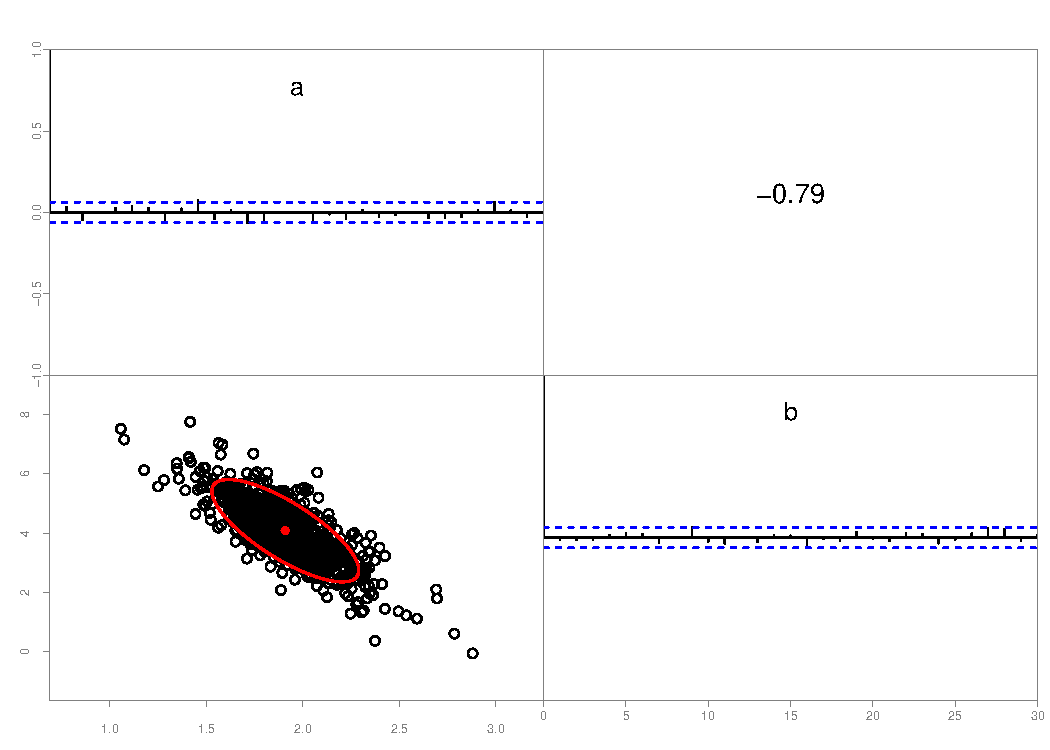
\includegraphics[width=5in]{../plots/simple2.pdf}
  \caption{The samples from a simple model with
    \texttt{mcsave}=100. Note the negligible autocorrelation
    of both parameters.The red ellipses show the estimated
    pairwise parameter covariances, and the red point the
    MPD.}
  \label{fig:simple2}
\end{figure}

\subsubsection{Opitmize the acceptance rate}
Studies have shown that there is an optimal range for
acceptance rate for the MH algorithm
(e.g. \cite{roberts2001}). If the proposal distribution
generates values too close to the current state, the chain
will accept them (high acceptance rate) but explore the
posterior slowly and need more thinning. Alternatively, if
proposals are too far away into regions of low density (low
acceptance rate) the chain will not explore the space. The
optimal acceptance rate varies by model, but is roughly
40\%. The general advice is to tune the proposal
distribution to achieve an efficient acceptance rate.

ADMB accomplishes this by ``scaling'' the covariance matrix
up or down, depending on the current acceptance rate, during
the first part of the chain. By default, it scales during
the first 500 iterations (and prints this to screen), but
the user can specify this with \texttt{mcscale N} or turn
off scaling with \texttt{mcnoscale}. ADMB rescales the
covariance matrix every 200 iterations until the acceptance
rate is between 0.15 and 0.4, or the scaling period is
exceeded.

In practice, the defaults work for many models, but the user
may want to extend the scaling period for some models. Draws
from this tuning phase should be discarded as part of the
burn-in.
\subsubsection{mcprobe}\label{sec:mcprobe}
\large{[if someone wanted to write this up more formally
  that'd be great]}
For some models, there may be concern of being ``stuck'' in
a local minimum and simply never proposing a value far
enough away to escape it and find other regions of high
density. ADMB has a built-in algorithm which modifies the
default proposal distribution so it occasionally proposes
very distant parameters (i.e. ``probes''). The
\texttt{mcprobe X}\footnote{Previous versions of ADMB called
  this \texttt{mcgrope} -- this is now deprecated} argument
initiates this option.

The modified proposal distribution is a mixture distribution
of normal and Cauchy distributions. The argument \texttt{X}
controls how the two distributions are mixed, with larger
values being more Cauchy (fatter tails) and lower being
thinner tails. The range of valid inputs is 0.00001 to
0.499, and if no value is supplied a default of 0.05 is
used\footnote{See the function for more information:
  \url{http://admb-project.org/documentation/api/prmonte\_8cpp\_source.html\#l00014}}

Figure \ref{fig:mcgrope_example} shows the shape of the
proposal distribution. Note the extremely fat tails, and
that the standard proposal itself is bounded.

\begin{figure}[h]
  \centering
  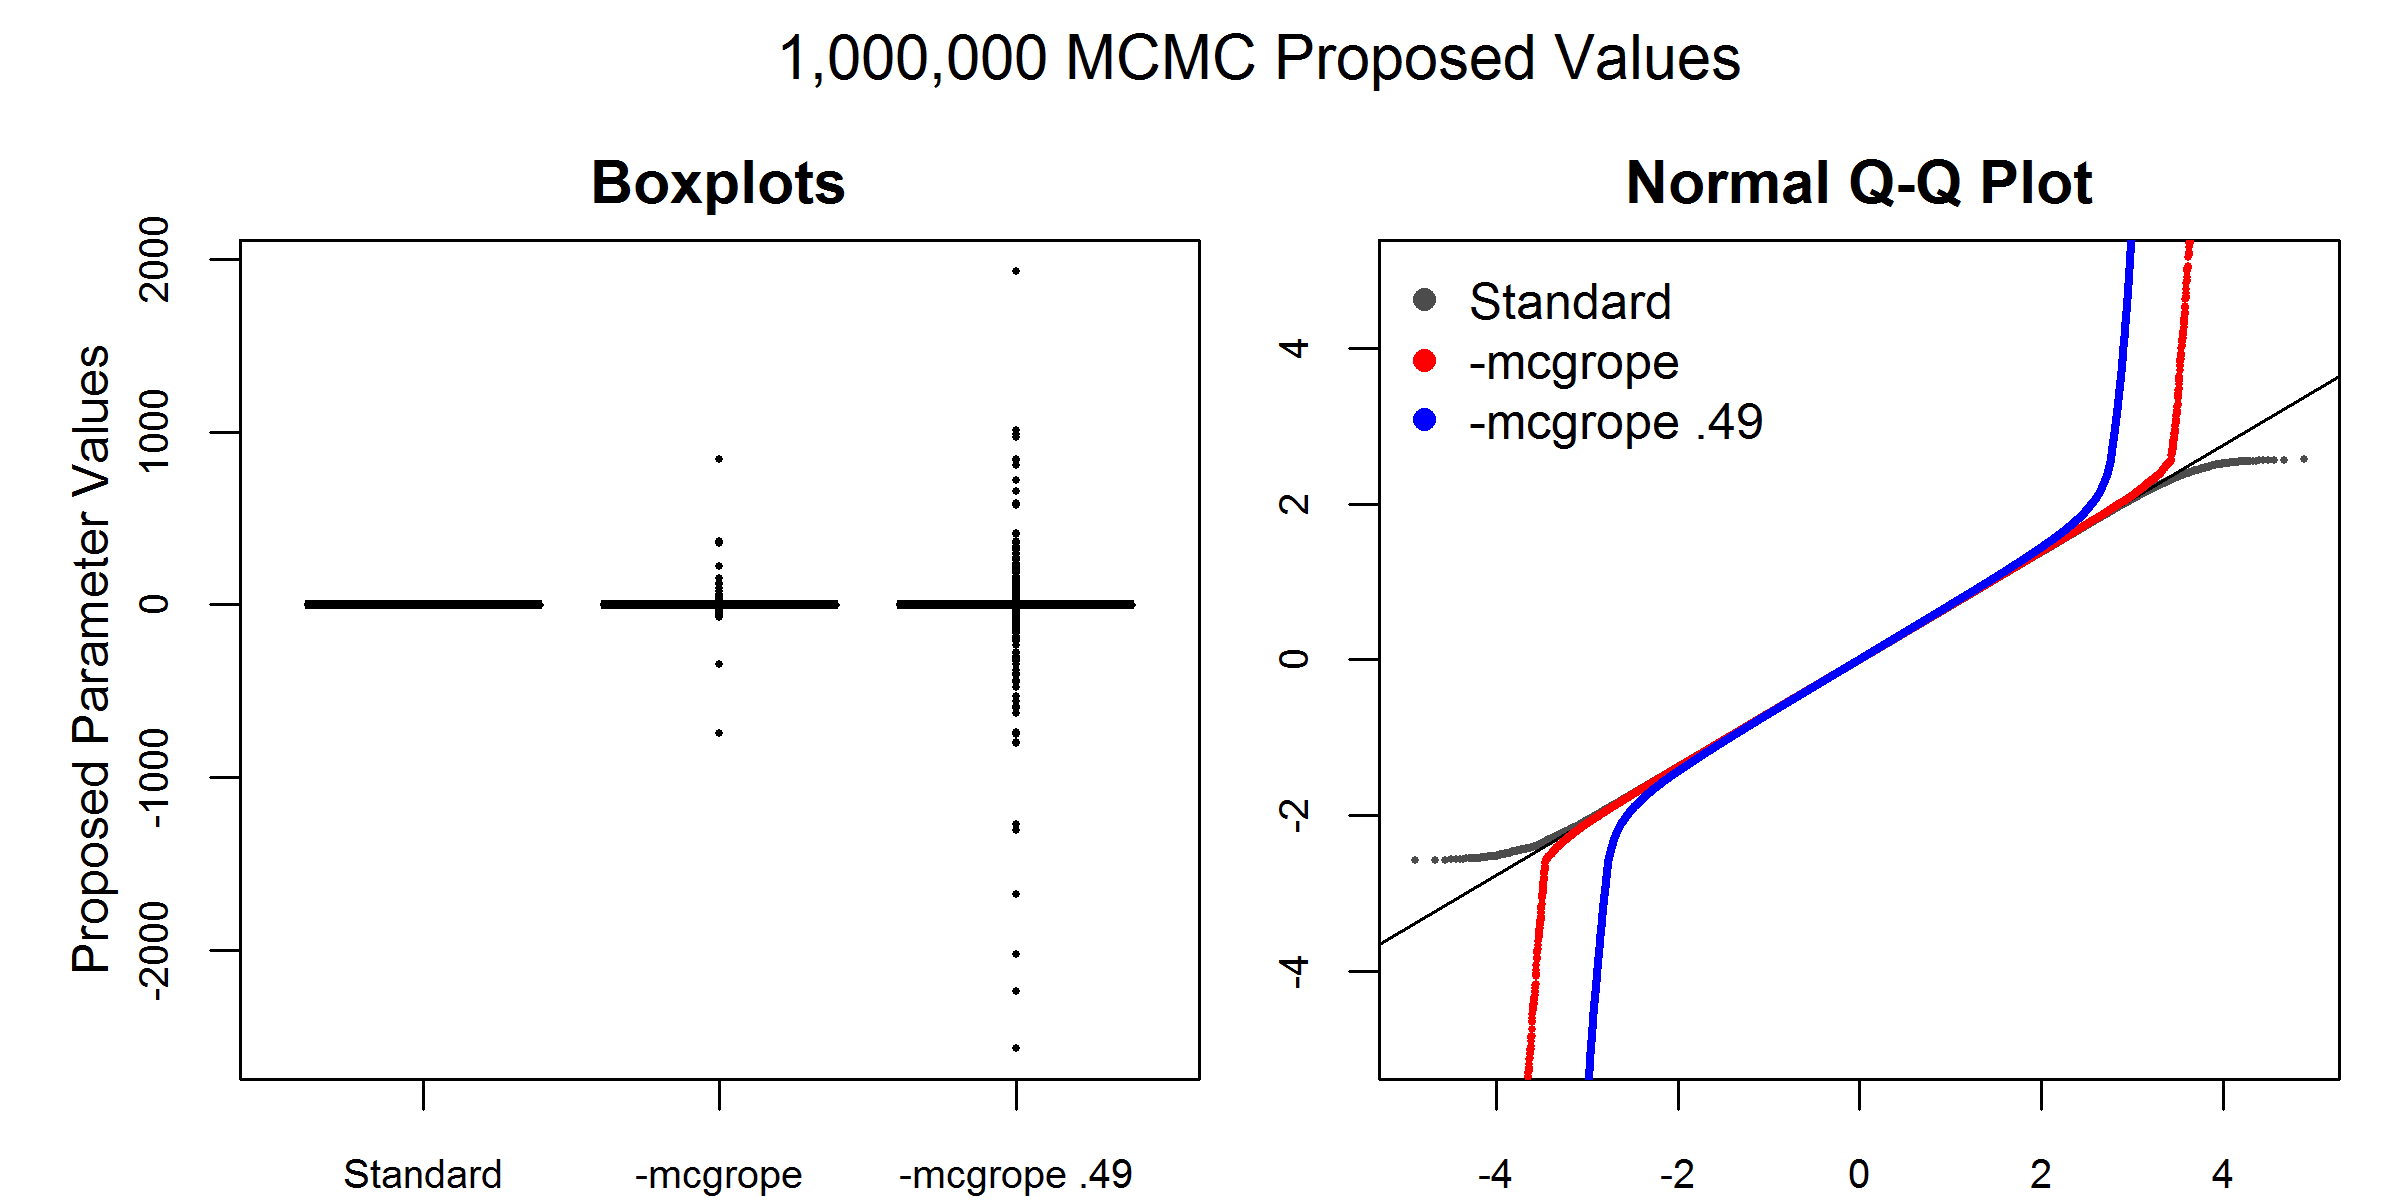
\includegraphics[width=5in]{../plots/mcgrope_example.png}
  \caption{Example of fat-tailed proposal values for a
    parameter for the \texttt{mcprobe} option compared to
    the default proposal.}
  \label{fig:mcgrope_example}
\end{figure}

\subsubsection{mcrb}\label{sec:mcrb}
The \texttt{-mcrb N} option (which stands for rescaled
bounded) alters the covariance matrix used to propose new
parameter sets in the MH algorithm. Its intended use is to
create a more efficient MCMC sampler so the analyses run
faster.

The option will be most effective under circumstances where
the correlation between parameters at the MPD is higher than
other regions of the parameter space. In this case, the
algorithm may make efficient proposals at the MPD, but
inefficient proposals in other parts of the space. By
reducing the correlation using \texttt{mcrb} the proposal
function may be more efficient on average across the entire
parameter space and require less thinning.


The \texttt{mcrb} option is a set of calculations performed
on the original correlation matrix, as follows.
\begin{align*}
  \mathbf{\Sigma_{\text{old}}}&=
  \begin{bmatrix}
    1 & \cdots & \rho_{1,n}\\
    \vdots & \ddots & \vdots\\
    \rho_{n,1} & \cdots & 1
  \end{bmatrix}
  \quad\text{The original correlation matrix}\\
  \mathbf{L}&=\begin{bmatrix}
    1 & \cdots & 0\\
    \vdots & \ddots & \vdots\\
    L_{n,1} & \cdots & L_{n,n}
  \end{bmatrix}
  \quad\text{Lower Choleski decomposition of $ \mathbf{\Sigma_{\text{old}}}$}\\
  \mathbf{\hat{L}}&=\begin{bmatrix}
    1 & \cdots & 0\\
    \vdots & \ddots & \vdots\\
    L_{n,1}^{N/10} & \cdots & L_{n,n}^{N/10}
  \end{bmatrix}
  \quad\text{Raise elements to power user supplied $N$}\\
  \mathbf{\tilde{L}}&=\begin{bmatrix}
    1 & \cdots & 0\\
    \vdots & \ddots & \vdots\\
    \frac{\hat{L}_{n,1}}{\left | \hat{L}_{n,\cdot}\right |} & \cdots &
    \frac{\hat{L}_{n,n}}{\left | \hat{L}_{n,\cdot}\right |}
  \end{bmatrix}
  \quad\text{Normalize rows of $\hat{L}$ }\\
  \mathbf{\Sigma_{\text{rb}}}&=\mathbf{\tilde{L}}\mathbf{\tilde{L}}^T
  \quad\text{Calculate new correlation matrix}
\end{align*}

By working with the Choleski decomposition of the
correlation matrix, the algorithm ensures that the rescaled
bounded matrix used in the MCMC remains a valid correlation
matrix (i.e. positive definite). The impacts on a
correlation matrix can be difficult to anticipate, but
fortunately ADMB writes the resulting covariance matrix to
the file \texttt{corrtest} (a text file with no ending)
under the label ``modified S''. The user can plot this
against the estimated covariance to visually gauge the
impact of the \texttt{mcrb} algorithm.

\begin{figure}[h]
  \centering
  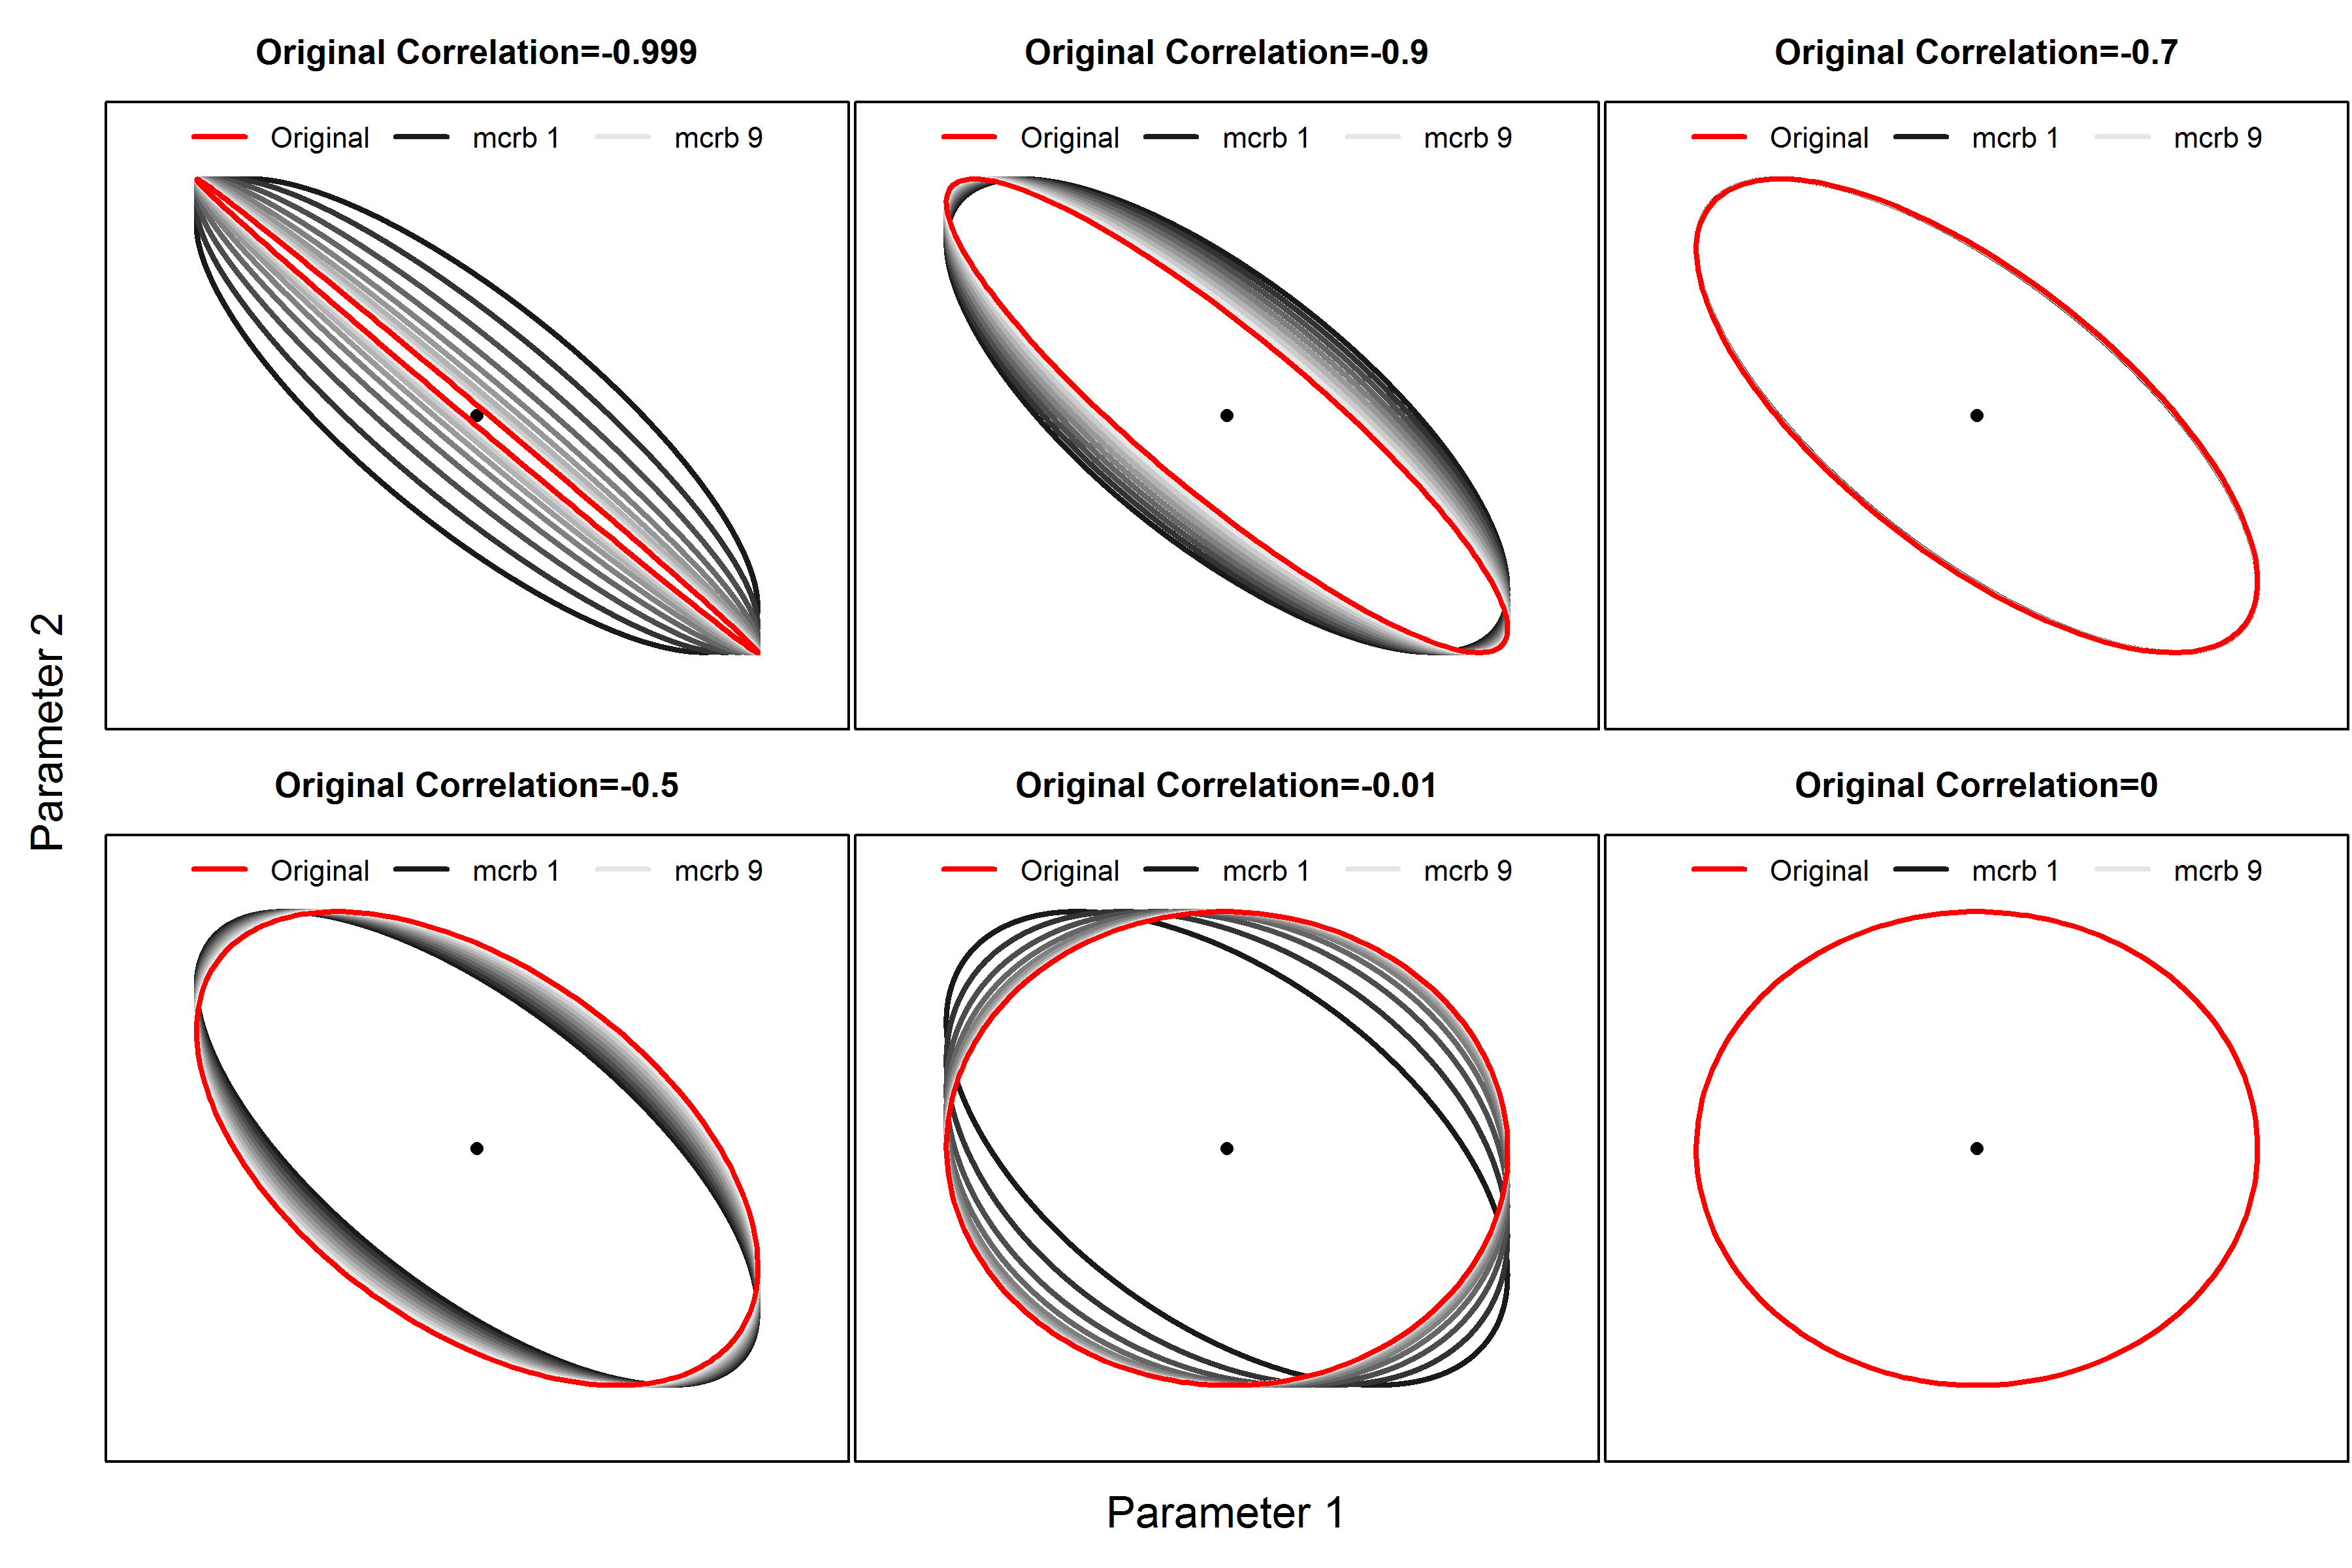
\includegraphics[width=5in]{../plots/mcrb_examples.png}
  \caption{The effect of \texttt{mcrb} on a variety of
    correlations between two hypothetical parameters. Note
    that the effect of setting $N=9$ depends on the original
    correlation.}
  \label{fig:mcrb}
\end{figure}

\subsubsection{User-supplied covariance matrix}\label{sec:user.cov}
The \texttt{mcrb} option is a quick way to try lowering the
correlation between some parameters. A more flexible (and
transparent) option is to provide ADMB with a covariance
matrix chosen by the user. By examining preliminary chains
or using information gained from other simple models, it may
be possible for the user to define a covariance matrix that
is more efficient than the estimated one, or modified via
the built-in options. We demonstrate the improved
perofrmance using this option in the next section.

Providing user-supplied covariance is a more advanced
technique that is not built in to ADMB. It requires a
slightly more detailed understand of the underlying output
file structure of ADMB. The steps to do this can be found in
the document at
\url{http://www.admb-project.org/examples/admb-tricks/covariance-calculations.}

\section{Hyrbid MCMC}\label{sec:hybrid}
The ``hybrid'' option in ADMB is an implementation of an
MCMC algorithm based on Hamiltonian dynamics. Here we provid
a simplified overview \footnote{Ignoring, for example, the
  transformation of the parameter space via the Choleski
  decomposition used by ADMB} of the algorithm, with the aim
of providing users an intuition about its behavior and
properties and how to use it within ADMB. This section is
based on \cite{brooks2011}, which provides a thorough review
of the algorithm, including background motivation, proof of
ergodicity, and illustrative examples\footnote{This chapter
  is available at
  \url{http://www.admb-project.org/developers/workshop/la-jolla-2010/ham-mcmc.pdf/view}}.

The hybrid method is different from the MH algorithm in how
it proposes new parameter values. Instead of proposing
random states based on the current value, the hybrid method
uses derivatives to follow a contour of the posterior
surface. By doing so, it (in theory) only proposes states
that are very likely to be accepted, and as such will have
less autocorrelation.

In some models, a well tuned hybrid chain will need less
thinning, if any at all, and run faster. The downside of the
algorithm is that it is more difficult to tune than the MH
algorithm.

\subsection{Algorithm}
The algorithm utilizes the properties of a physical system
known as Hamiltonian dynamics. Hamiltonian dynamics, while
based in physics, provides some extremely useful
mathematical properties for Bayesian integration via MCMC.

A Hamiltonian system consists of two parameter vectors of
equal length: ``position'' ($\mathbf{q}$) and ``momentum''
($\mathbf{p}$). How these parameters change over time is
described by the Hamiltonian function,
$H(\mathbf{q},\mathbf{p})$. This system can be
conceptualized as a frictionless surface about which an
object moves. At some time $t$ an object has a certain
height (position) and momemtum. The height of the surface is
equal to the objective function of our model, and the
momentum variables are introduced parameters to ensure the
Hamiltonian dynamics are met. Samples from a posterior are
generated by simulating the object moving about the joint
surface through time, governed by $H$.

For use with MCMC, $H$ is assumed to be
$H(\mathbf{q},\mathbf{p})=U(\mathbf{q})+K(\mathbf{p})$,
where $U$ is analagous to the potential energy and $K$
kinetic energy. $U$ is set equal to the ADMB objective
function (i.e. the negative log of the posterior density)
and $K$ to a diagonal multivariate normal distribution. The
hybrid MCMC algorithm samples from the joint posterior, $H$,
but we are only interested in the posterior for $U$, so $K$
is not saved by ADMB.

The time trajectory of the object through the joint
probability space, $H$, is used to generate proposed
parameter sets. Given the form for $H$ above, the
fundamental equations of motion are:
\begin{align}
  \label{eq:motion}
  \frac{dq_i}{dt} &= \frac{\partial{K}}{\partial{p_i}}\\
  \frac{dp_i}{dt} &= -\frac{\partial{U}}{\partial{q_i}}
\end{align}

ADMB uses the ``leapfrog'' method to discretize equations
\eqref{eq:motion}. The leapfrog method is more reliable than
the well-known Euler method. It has two tuning parameters:
the number of steps to take (\texttt{hynstep}), and the step
size $\varepsilon$ (\texttt{hyeps}). The following sequence of
calculations shows a single iteration of the leapfrog
method, for the $i^{\text{th}}$ variable, and is repeated
\texttt{hynstep} times sequentially.
\begin{align*}
  p_i(t+\varepsilon/2)&=p_i(t)-(\varepsilon/2)\frac{\partial{U}}{\partial{q_i}}q(t)\\
  q_i(t+\varepsilon)&=q_i(t)+\varepsilon \frac{p_i(t+\varepsilon/2)}{mi}\\
  p_i(t+\varepsilon)&=p_i(t+\varepsilon/2)-(\varepsilon/2)\frac{\partial{U}}{\partial{q_i}}q(t+\varepsilon)
\end{align*}

The leapfrog algorithm moves deterministically through the
joint surface along a contour of (appoximately) constant
$H$. That is, for a given starting value of $(q_0,p_0)$ and
tuning parameters the trajectory will always end in the same
place. Examples of trajectories under different tuning
parameters for the leapfrog method are given in figure
\ref{fig:hybrid_grid_trace}. Note that ADMB calculates the
partial derivatives $\frac{\partial{U}}{\partial{q_i}}$ at
each function evaluation using automatic
differentiation. Thus these are available for any model and
do not have to be determined analytically, which can be
difficult or impossible for large, non-linear models.

\begin{figure}[h]
  \centering
  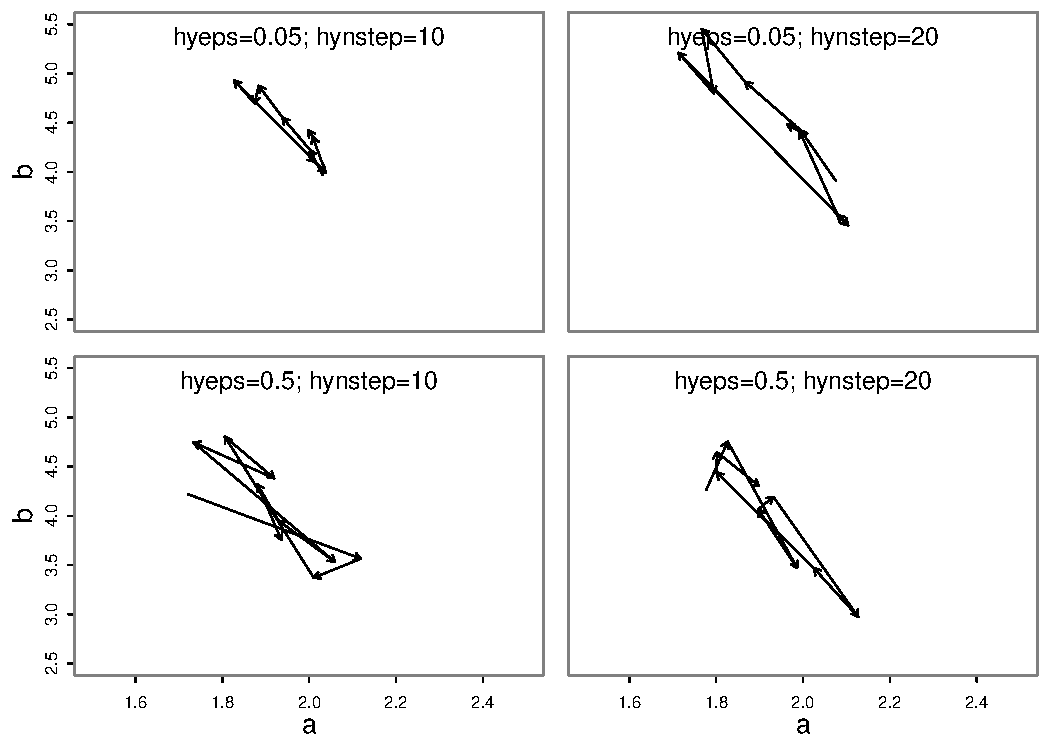
\includegraphics[width=5in]{../plots/hybrid_grid_trace.pdf}
  \caption{Leapfrog trajectories for different sets of
    tuning parameters. The posterior surface is shown as
    contours, and the posterior mode as a red point. The
    filled black point is the starting point, and the arrows
    show the trajectory of the leapfrog steps, ending at the
    open circle representing the proposed set of
    parameters.}
  \label{fig:hybrid_grid_trace}
\end{figure}

Casting a posterior into a Hamiltonian system and
discretizing it with the leapfrog method is simply a way to
generate proposed sets of parameters in the larger,
stochastic MCMC algorithm. A single iteration of the hybrid
MCMC algorithm, as implemented in ADMB, has three steps:
\begin{enumerate}
\item \textbf{Propose new momentum variables.} New momentum
  values, $p^*$ are generated from a normal distribution
  based on the estimated covariance matrix, and independent
  of the current position variables.
\item \textbf{Propose new position variables.} Given the
  current state of the system, $(q,p^*)$, new position
  variables $q^*$ are generated with the leapfrog algorithm
  using \texttt{hynstep} \footnote{Actually a random
    integers is generated around this value} steps and a
  step size of \texttt{hyeps}.
\item \textbf{Accept or reject the new state.} The new state
  is then updated with a Metropolis step (i.e. accepted or
  rejected) in the same way as above. Acceptance is expected
  to be high because the proposed values $(q^*, p^*)$ are
  rarely into regions of low density for a well tuned chain.
\end{enumerate}

We can see the first two steps of the algorithm by randomly
drawing values for $U$ and doing a leapfrog projection to
the proposed parameters (Fig. \ref{fig:hybrid_seeds}).
\begin{figure}[h]
  \centering
  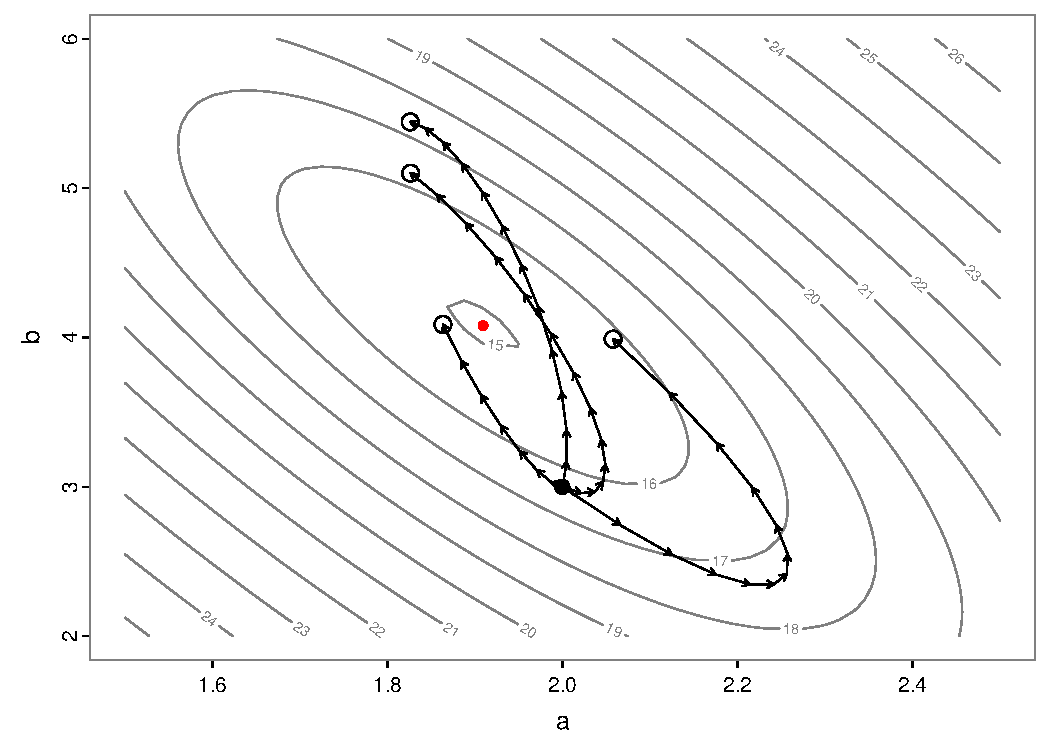
\includegraphics[width=5in]{../plots/hybrid_seeds.pdf}
  \caption{Leapfrog projections for different random draws
    from $U$.}
  \label{fig:hybrid_seeds}
\end{figure}

A perhaps intuitive question might be: why bother with the
momentum variables at all? One issue is that without the
momentum variables, and the Hamiltonian dynamics in general,
we would need to account for changes in volume in the
acceptance probability (step 3 above)\cite{brooks2011}. This
would require computing the determinant of the Jacobian
matrix of the mapping defined by the dynamics. This Jacobian
is not readily available and is often computationally
intensive. Thus the need to adopt the Hamilton dynamics
framework.  Hamiltonian dynamics also provides other
properties required for an ergodic Markov chain
\cite{brooks2011}.

The hybrid MCMC thus samples from the joint posterior of the
position and momentum vectors, but ADMB discards the
momentum variables and returns only the position
variables. The user can then do inference on those samples
in the same was as the Metropolis-Hastings method, given
they come from a properly converged (stationary) chain.

\subsection{Arguments}
Arguments for the hybrid algorithm are in general similar to
those above, so we only discuss the differences. The main
arguments are:
\begin{table}[H]
  \centering
  \begin{tabular}[h]{|cl|}
    \hline
    \texttt{-mcmc N} & Run $N$ MCMC iterations\\
    \texttt{-hybrid} & Use the hybrid method\\
    \texttt{-hynstep N} & Mean number of steps for the leapfrog method\\
    \texttt{-hyeps X} & The stepsize for the leapfrog method [X numeric and $>0$]\\
    \hline
  \end{tabular}
  \caption{ADMB runtime arguments for the hybrid MCMC}
  \label{tab:hy_args}
\end{table}
Since the estimated covariance matrix is used in the
algorithm, the \texttt{mcdiag}, \texttt{mcrb N}, and
\texttt{mcmult} options above are also available. The
\texttt{mcprobe} argument is not currently supported for the
hybrid algorithm.

Note that \texttt{mcsave N} is \textbf{not} an argument for
the hybrid and will be ignored. Each MCMC iteration of the
hybrid algorithm is saved, such that the user may need to
thin the chain manually after running.

\subsection{Tuning the hybrid algorithm}
A tuned hybrid MCMC algorithm often provides a more
efficient (computationally) chain than the random walk
behavior of the Metropolis-Hastings algorithm. However, the
hybrid algorithm is often much more difficult to tune. A
thorough review of tuning techniques is beyond the scope of
this guide, and we refer users to \cite{brooks2011} for
further reading of more advanced tuning techniques and
intuition about reasonable values\footnote{The ADMB
  algorithm works in the transformed space, via the Cholesky
  decomposition of the estimated covariance matrix, making
  intuition about tuning even more difficult}.

In most practical applications the hybrid method is tuned
via trial and error. That is, values for \texttt{hynstep}
and \texttt{hyeps} are tried on a short chain, and the
output diagnosed. ADMB uses default values of 0.1 and 10,
respectively, and these may be good starting values for most
problems. The end goal is to find a set of tuning parameters
that produces a well mixing chain with the fewest leapfrog
steps. Figure \ref{fig:hybrid_grid_acf} shows the
autocorrelation of a parameter from the simple model across
different tuning parameters. Note that the top right and
bottom left panels show very similar ACF patterns, which
should not be a surprise when compared to the corresponding
leapfrog trajectories in
\ref{fig:hybrid_grid_trace}. Further, from that figure we
can see that a chain with a \texttt{hynstep} of 100 cycles
the surface many times, and although it mixes well, this
value could probably be lowered and the runtime reduced
without affecting mixing. This is somewhat analagous to
having a higher thinning rate than is necessary.

\begin{figure}[h]
  \centering
  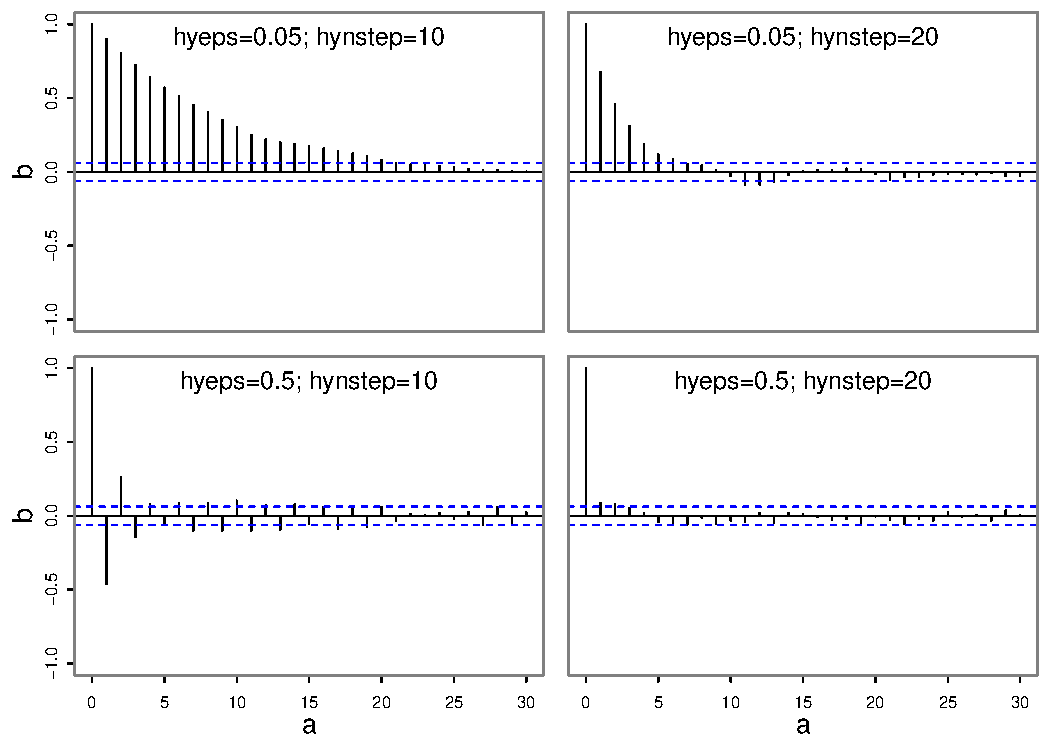
\includegraphics[width=5in]{../plots/hybrid_grid_acf.pdf}
  \caption{The autocorrelation of the parameter $a$ from the simple model
    across different tuning parameters of the hybrid method.}
  \label{fig:hybrid_grid_acf}
\end{figure}

A word of caution regarding the tuning of hybrid chains. For
most values of \texttt{hyeps} the leapfrog trajectories will
be ``stable'' in that they will cycle around a contour of
$H$ (this can be seen in the last panel in figure
\ref{fig:hybrid_grid_trace}). However, for values of
\texttt{hyeps} that are too large, the method becomes
unstable and trajectories diverge ($H$ is no longer
constant), causing the algorithm to propose parameters with
low density which are then rejected. Unfortunately for real
problems, the value of \texttt{hyeps} that is``too big'' can
vary across the posterior space.  Another issue that can
arise is that certain combinations of tuning parameters can
lead to near periodicity. That is, the leapfrog trajectory
ends very near to where it began, after one or more
steps. In pathological cases it could cycle forever and
never be able to sample regions of the posterior space
(i.e. not be ergodic). In practice near periodicity will
make for a very slow mixing chain. ADMB mitigates this
possibility by randomly drawing the number of leapfrog steps
at each MCMC iteration. However, the user should still be
aware of these potential issues and be vigilant in
diagnosing the mixing behavior of a hybrid chain. Samples
from an MCMC chain that is not in equilibrium, or has other
issues, can lead to incorrect inference.

\section{An example with non-linear posterior}
The simple example used above had the characteristic that
the parameters were correlated, but this correlation was
constant across the entire posterior. Thus the same proposal
distribution worked well throughout the parameter space.

Here we look at another example with two parameters, but
where the correlation changes. This example uses contrived
data and a discrete theta-logistic model. This is a classic
example of a simple model which can lead to convergence
issues for MCMC chains.

We first run it with the default settings and a thinning
rate of \texttt{mcsave}=100.

\begin{figure}[h]
  \centering
  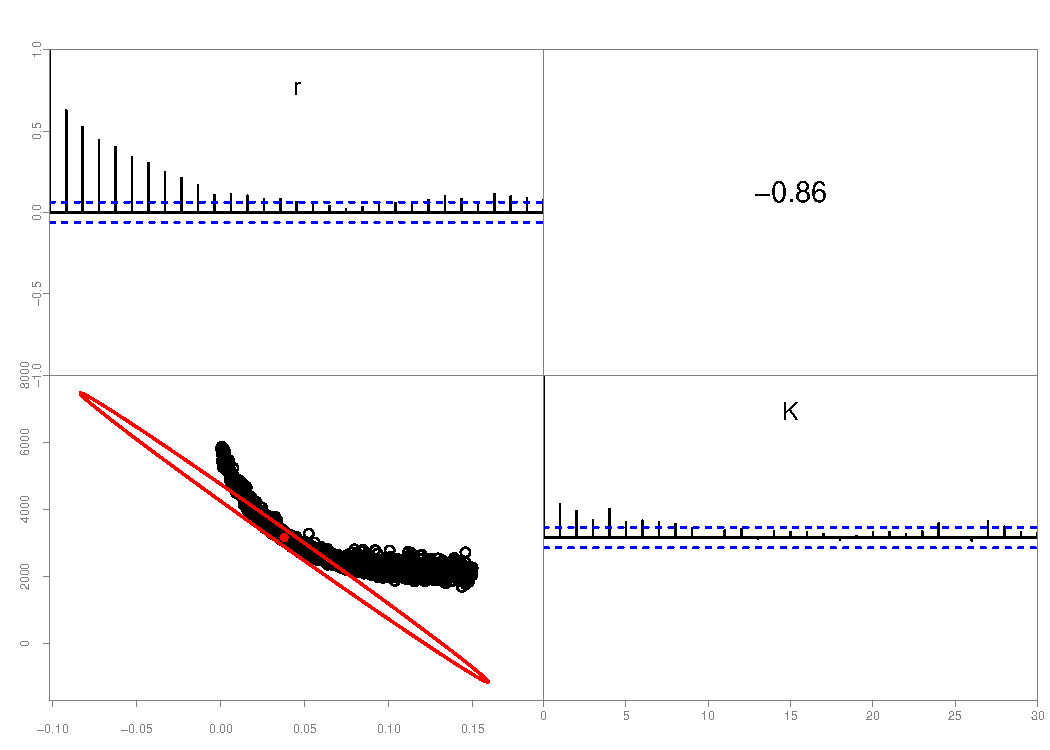
\includegraphics[width=5in]{../plots/logistic_mh.pdf}
  \caption{The logistic model with 1 in 100 samples saved
    using the MH algorithm and estimated covariance matrix
    (red ellipse).}
  \label{fig:logistic_mh}
\end{figure}
We can immediately see the autocorrelation remains high even
after thinning. One option would be to increase the thinning
rate. Another is to try a lower correlation. From this
initial run we calculate the empirical covariance matrix and
rerun the chain with this option (see \ref{sec:user.cov}).

\begin{figure}[h]
  \centering
  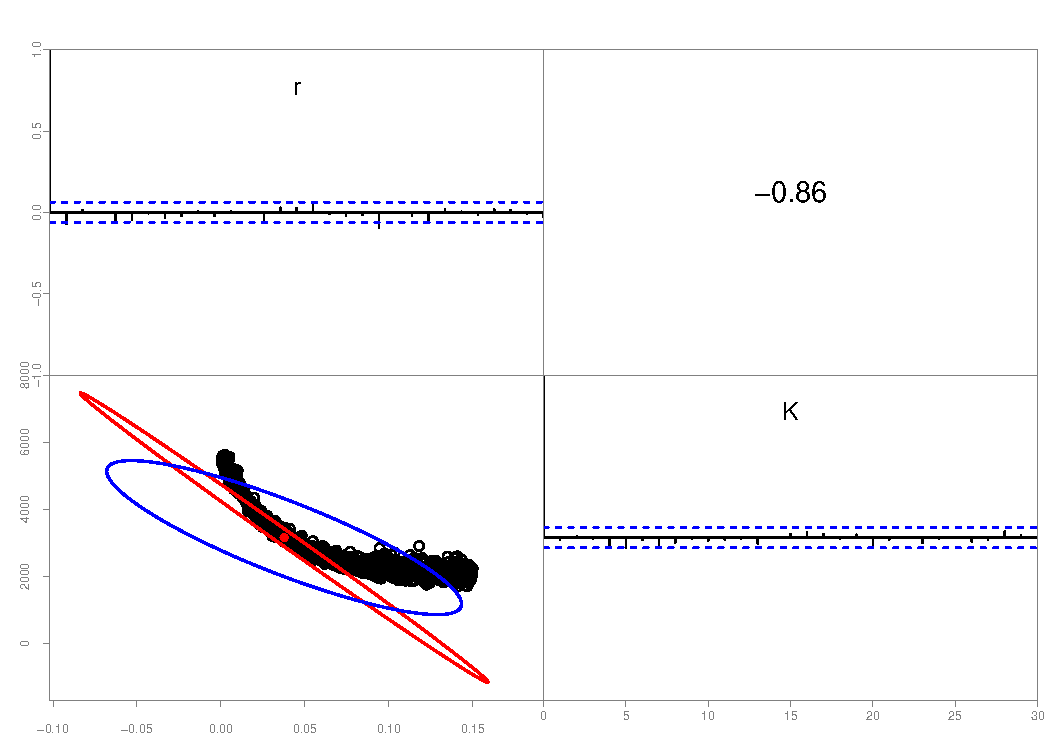
\includegraphics[width=5in]{../plots/logistic_mh2.pdf}
  \caption{The logistic model with 1 in 100 samples saved
    using the MH algorithm and empirical covariance matrix
    (blue ellipse). Note the improvement in acf compared to
    \ref{fig:logistic_mh}.}
  \label{fig:logistic_mh2}
\end{figure}
Here we see a substantial improvement in the chain
performance by changing the proposal distribution of the
Metropolis-Hastings algorithm. This option is far superior
to increasing the thinning rate because it takes no more
time to run.

We can also try the hybrid algorithm on this model, starting
with the default parameters of \texttt{hyeps} and
\texttt{hynstep} of 0.1 and 10, and using the estimated
covariance matrix.
\begin{figure}[h]
  \centering
  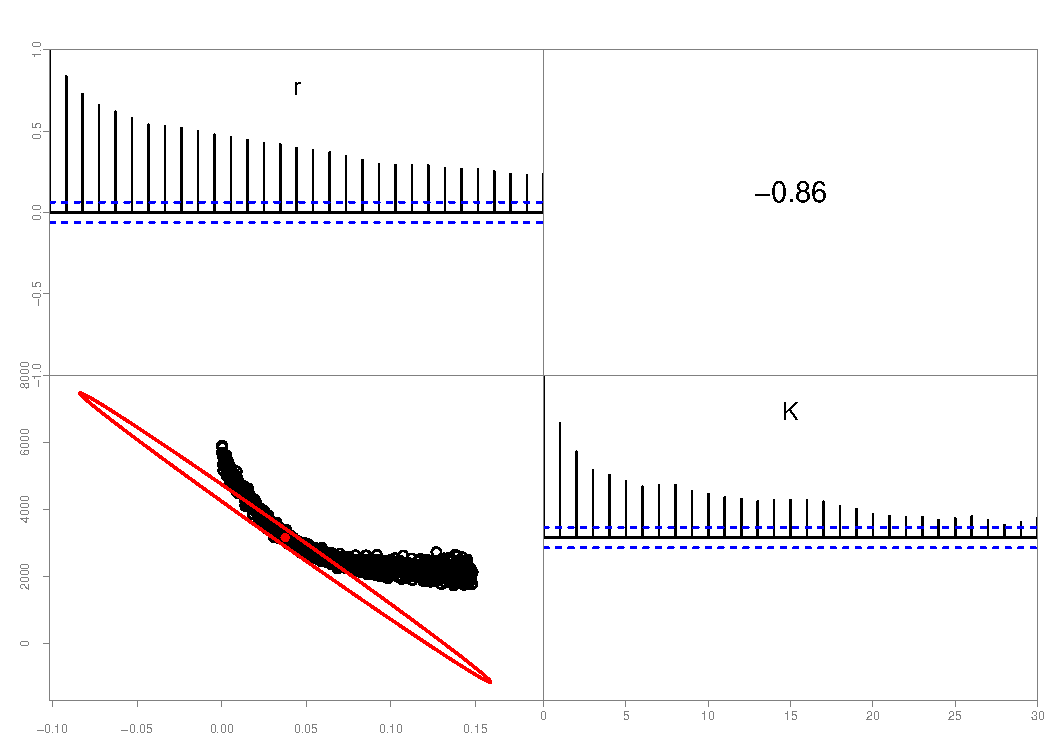
\includegraphics[width=5in]{../plots/logistic_hy.pdf}
  \caption{The logistic model using the hybrid method with
    default tuning parameters and the estimated covariance matrix
    (red ellipse).}
  \label{fig:logistic_hy}
\end{figure}
The autocorrelation is high, suggesting we need to tune the
chain. First we try the same as above, and instead use the
empirical covariance matrix.
\begin{figure}[h]
  \centering
  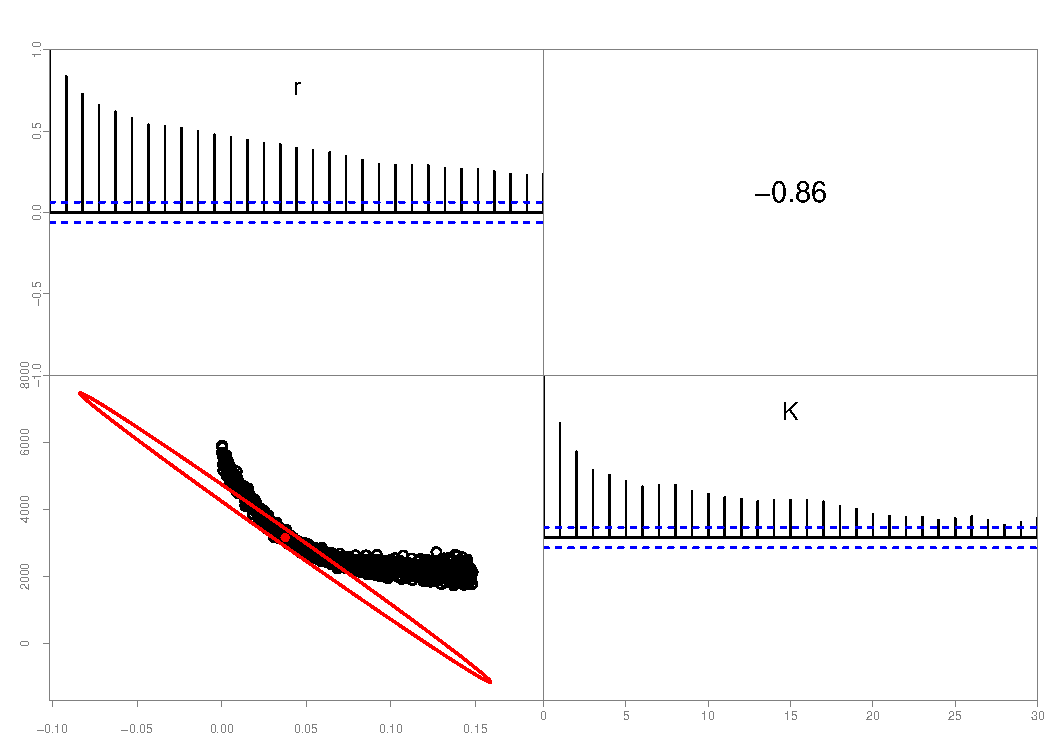
\includegraphics[width=5in]{../plots/logistic_hy.pdf}
  \caption{The logistic model using the hybrid method with
    default tuning parameters and the empirical covariance matrix
    (blue ellipse).}
  \label{fig:logistic_hy2}
\end{figure}
This chain is performing better, but is still
autocorrelated. A little trial and error the combination of
\texttt{hyeps 0.05} and \texttt{hynstep 100} performed
significantly better, and similarly to the tuned MH chain in
\ref{fig:logistic_mh2}.
\begin{figure}[h]
  \centering
  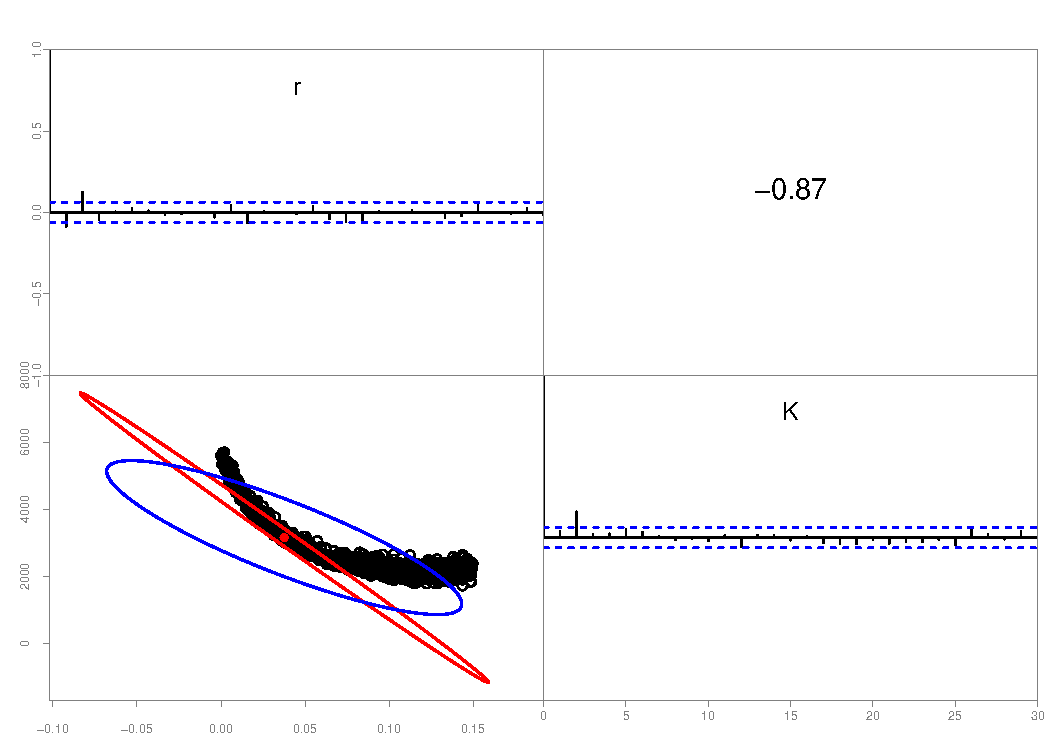
\includegraphics[width=5in]{../plots/logistic_hy3.pdf}
  \caption{The logistic model using the hybrid method and
    \texttt{hyeps 0.05} and \texttt{hynstep 100} for tuning
    parameters and the empirical covariance matrix (blue
    ellipse).}
  \label{fig:logistic_hy3}
\end{figure}

Here the hybrid and MH perform similarly with the same
number of function evaluations per sample (\texttt{hynstep}
and \texttt{mcsave}, respectively). With a little trial and
error, and visual exploration of the posterior surface it
was fairly straightforward to improve on the default
performance. It is likely possible to further refine the
hybrid algorithm to outperform the MH, but it is not clear
which of the parameters to start with. The difficulty in
tuning

For many problems, the default MH algorithm will work well
and require no tuning beyond a modest thinning rate. We
encourage users to start with this algorithm, and explore
alternatives only if computational efficiency is restrictive
for the needs at hand. The hybrid method is more
sophisticated, but much more difficult to tune, and we
recommend it as an option only when the MH is struggling.

\newpage
\bibliographystyle{unsrt}
\bibliography{admb_guide}.
\end{document}


